\subsection{Sofware environment}
\label{subsec:3.1}
INT2LM  and the  COSMO-ART model  are  implemented in  Fortran 90  for
distributed  memory  parallel  computers  using  the  Message  Passing
Interface (MPI).   The software stack on both  many-core platforms was
controlled  using  the  modules  framework  which gives  an  easy  and
flexible mechanism  to access to  all of the CSCS  provided compilers,
tools and  applications.  For our  initial benchmarking, we  opted for
the GNU compiler  (gcc/4.8.1 on Monch, gcc/4.8.2 on  Pilatus) with the
-O3 compiler flag  as it generally gives a  good level of optimization
and the code runs faster in this configuration than when compiled with
the  intel  compiler  (14.0.1).   Besides,  we  installed  the  MPICH2
implementation of MPI (mvapich2/1.9) as well as the commonly used HDF5
(1.8.12) and NetCDF (4.3.1) libraries in favor of the traditional GRIB
library  for  the  management  of  extremely large  and  complex  data
collections.   The Linux  kernels  ``2.6.32-358.11.1.el6.x86\_64'' and
``3.0.101-0.15-default'' were  used as compute nodes OS  for Monch and
Pilatus respectively.

\subsection{Run configuration}
\label{subsec:3.2}
The COSMO-ART model uses NAMELIST-input to specify runtime parameters
splitted into several groups (see Table~\ref{tab:1}). 

\begin{table}[htbf]
  \begin{center}
    \caption{}
    \label{tab:1}
    \begin{tabular}{ll}
      \hline\noalign{\smallskip} 
      \textbf{Group} & \textbf{Description} \\
      \noalign{\smallskip}\hline\noalign{\smallskip}
      LMGRID & Grid domain and size parameters \\
      RUNCTL & Model run parameters \\
      TUNING & Physics and dynamics parameters \\
      DYNCTL & Adiabatic model parameters \\
      PHYCTL & Diabatic model parameters \\
      COSMO\_ART & Gases and aerosols model parameters \\
      DIACTL & Diagnostic calculations parameters \\
      SATCTL & Synthetic satellite images parameters \\
      IOCTL & I/O environment parameters \\
      GRIBIN & GRIB input parameters \\
      GRIBOUT & GRIB output parameters \\
     \noalign{\smallskip}\hline
    \end{tabular}
  \end{center}
\end{table}

\noindent
In  particular,  to  run   COSMO-ART  the  following  input  data  are
necessary:
\begin{itemize}
\item  Gas phase:  Anthropogenic emissions  for different  species and
  land use data for biogenic emissions and deposition,
\item Aerosol particles: Anthropogenic emissions,
\item Mineral dust: Soil specific land use data.
\end{itemize}

A snapshot of the code, which includes, at least conceptually, all the
information needed  to reproduce the  energy-to-solution benchmarks of
COSMO-ART, was  produced and run on a  full rack of 52  nodes on Monch
(monchc[029-080]), i.e.  a total of 1040 cores using 20 tasks per node
and on  a full rack of  42 nodes on Pilatus  (pilatus[03-44]), i.e.  a
total of  1344 cores using 16  tasks per node.   The calculated region
was  mapped to  the participating  processors using  a 2D-partitioning
strategy.  The distribution along the  x and y coordinates was defined
by setting: $nprocx=40$ and  $nprocy=26$ for Monch and $nprocx=28$ and
$nprocy=24$.  Besides as this version of COSMO-ART doesn't make use of
the   GRIB   library,  we   specified   $nprocio=0$   for  GRIB   I/O.
Hyperthreading is not considered in this study as previous attempts of
its use revealed that it always led to higher energy-to-solution.\\

Multiple production runs of COSMO-ART were performed to illustrate the
reproducibility  of   the  baseline,  and   quantify  the  significant
uncertainties in  the power measurement, as dictated  by the available
technology (see subsection~\ref{subsec:2.2}).

\subsection{Power-measurement results}
\label{subsec:3.3} 
The  computing performance  and  energy efficiency  evaluation of  the
aforementioned   platforms  is   involving   two  important   metrics:
\textit{time-to-solution}       and       \textit{energy-to-solution}.
Time-to-Solution  refers to  the total  wall clock  time spent  by the
application  to  obtain results,  which  in  our  case represents  the
overall execution time of  COSMO-ART. Energy-to-solution is the amount
of energy spent to achieve  results. We present here an approach which
consists  in measuring the  power consumption  on one  entire cabinet.
The  sampled  instantaneous power  during  execution  is averaged  and
multiplied by the time-to-solution to determine energy-to-solution.

\begin{figure}[htbf]
  \begin{center}
    \includegraphics[width=0.48\textwidth]{Figs/NRJ_benchmark_Monch.eps}
    \caption{Monch: Isola E1 Rack 2 Total Power and Isola E1 Total
      Power}
    \label{fig:1}
  \end{center}
\end{figure}

\begin{figure}[htbf]
  \begin{center}
    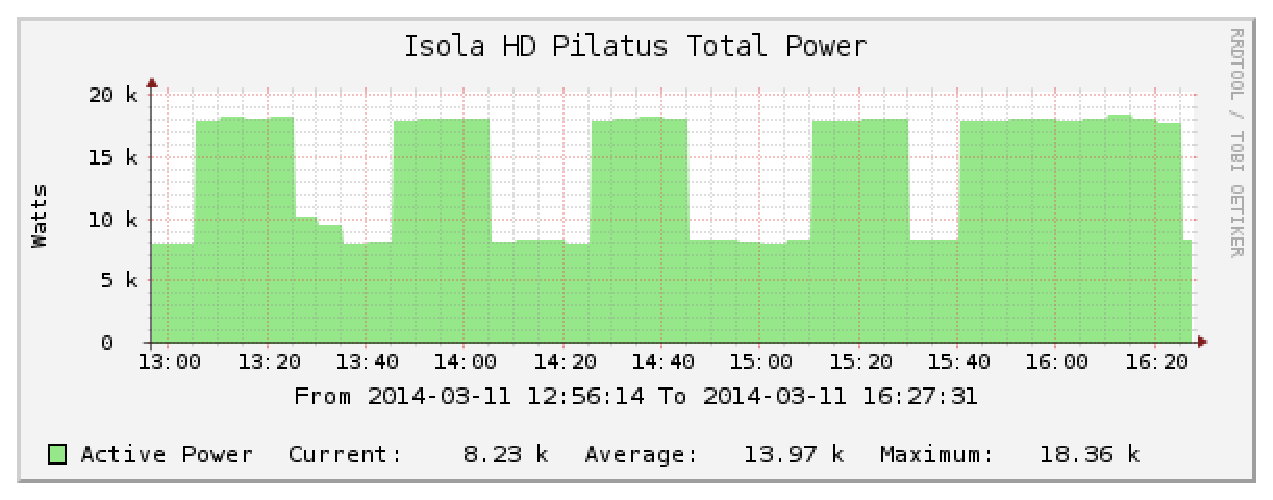
\includegraphics[width=0.48\textwidth]{Figs/NRJ_benchmark_Pilatus.eps}
    \caption{Pilatus: Isola HD Total Power}
    \label{fig:2}
  \end{center}
\end{figure}

Figures~\ref{fig:1} and  \ref{fig:2} account respectively  for Monch's
Isola E1  Rack 2  and Pilatus' Isola  HD total power  measurements for
1-day or 2-days simulations. On  the Intel Ivy Bridge EP based cluster
(i.e. Monch), the 1-day simulation  was issued only twice due to usage
restrictions. As time resolution was set to one update every 5 minutes
for  power sampling,  the average  power consumption  was  computed by
considering 6 values for each single  run.  On the Intel Xeon E5 based
cluster (i.e.   Pilatus), the 1-day  simulation was issued  four times
and a 2-days  run only once. Similarly, the  average power consumption
was computed by  considering 4 values for each single  1-day run and 9
values  for the  2-days  run. Corresponding  results  are gathered  in
Table~\ref{tab:3}.

\begin{table}[htbf]
  \begin{center}
    \caption{Average power consumption (W) of the platforms}
    \label{tab:3}
    \begin{tabular}{ccc}
      \hline\noalign{\smallskip}
      \textbf{Simulation time} & \textbf{Xeon E5} & \textbf{Ivy Bridge EP} \\
      \noalign{\smallskip}\hline\noalign{\smallskip}
      \textbf{1 day} & 18122.01417 & 12658.52278 \\ 
      & 17979.61083 & 12586.40833 \\
      & 18065.45167 & - \\
      & 17973.02833 & - \\
      \noalign{\smallskip}\hline\noalign{\smallskip}
      \textbf{2 days} & 17997.57815 & - \\
      \noalign{\smallskip}\hline
    \end{tabular}
  \end{center}
\end{table}

In Figure~\ref{fig:3}, we compare both time-to-solution (right y-axis)
and  energy-to-solution (left  y-axis) metrics  on both  platforms. As
expected, the 1-day  simulation on Ivy Bridge EP  presents the highest
execution time being roughly 1.3x  slower than Xeon E5. The reason for
that is  twofold: (i) it has  lower clock frequency than  Xeon E5 (2.2
GHz against 2.6 GHz); (ii)  Xeon E5 is a performance-centric processor
that is  tuned far more speed  than for low power  consumption. In our
experiments,  Ivy  Bridge   EP  showed  the  best  energy-to-solution,
reducing the energy consumption of Xeon E5 by approximately $7\%$.

\begin{figure}[htbf]
  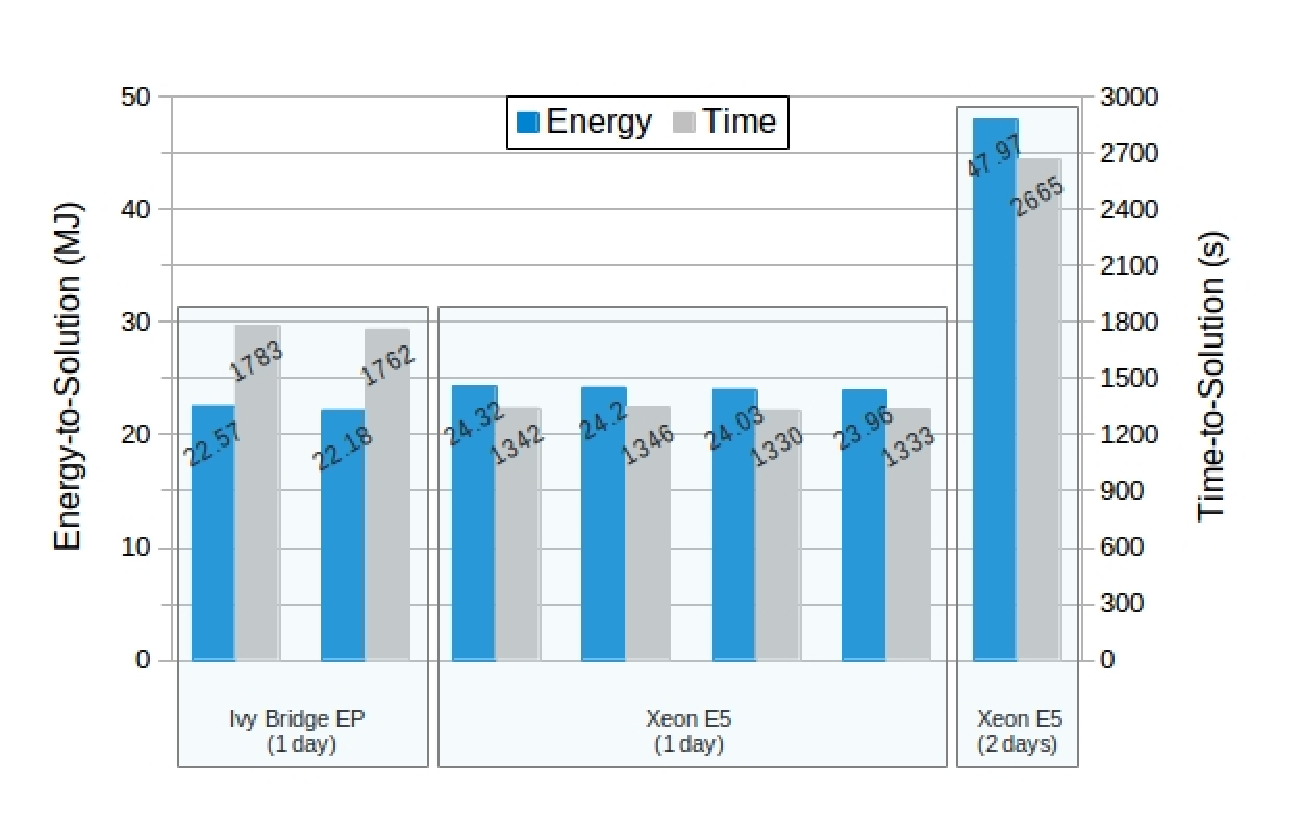
\includegraphics[width=0.5\textwidth]{Figs/Time_E2S_COSMO-ART.eps}
  \caption{Time and energy-to-solution comparison between Xeon E5 and
    Ivy Bridge architectures}
  \label{fig:3}
\end{figure}
